\documentclass[letterpaper,final,12pt,reqno]{amsart}

\usepackage[total={6.3in,9.2in},top=1.1in,left=1.1in]{geometry}

\usepackage{times,bm,bbm,empheq,fancyvrb,graphicx}
\usepackage[dvipsnames]{xcolor}
\usepackage{longtable}

\usepackage{tikz}
\usetikzlibrary{decorations.pathreplacing}

\usepackage[kw]{pseudo}
\pseudoset{left-margin=15mm,topsep=5mm,idfont=\texttt}

% hyperref should be the last package we load
\usepackage[pdftex,
colorlinks=true,
plainpages=false, % only if colorlinks=true
linkcolor=blue,   % ...
citecolor=Red,    % ...
urlcolor=black    % ...
]{hyperref}

\renewcommand{\baselinestretch}{1.05}

\newtheorem{lemma}{Lemma}

\newcommand{\Matlab}{\textsc{Matlab}\xspace}
\newcommand{\eps}{\epsilon}
\newcommand{\RR}{\mathbb{R}}

\newcommand{\grad}{\nabla}
\newcommand{\Div}{\nabla\cdot}
\newcommand{\trace}{\operatorname{tr}}

\newcommand{\hbn}{\hat{\mathbf{n}}}

\newcommand{\bb}{\mathbf{b}}
\newcommand{\bbf}{\mathbf{f}}
\newcommand{\bg}{\mathbf{g}}
\newcommand{\bn}{\mathbf{n}}
\newcommand{\bu}{\mathbf{u}}
\newcommand{\bv}{\mathbf{v}}
\newcommand{\bw}{\mathbf{w}}
\newcommand{\bx}{\mathbf{x}}

\newcommand{\bV}{\mathbf{V}}
\newcommand{\bX}{\mathbf{X}}

\newcommand{\bxi}{\bm{\xi}}

\newcommand{\bzero}{\bm{0}}

\newcommand{\rhoi}{\rho_{\text{i}}}

\newcommand{\ip}[2]{\left<#1,#2\right>}

% numbering
\setcounter{tocdepth}{3}
\makeatletter
\def\l@subsection{\@tocline{2}{0pt}{4pc}{5pc}{}}
\makeatother

\numberwithin{equation}{section}
\numberwithin{figure}{section}
\numberwithin{table}{section}


\begin{document}
\title[Geometric multigrid for glacier modeling]{Geometric multigrid for glacier modeling: \\ A Review and User's Guide}

\author{Ed Bueler}

\begin{abstract} FIXME: two principles in introduction: mass conservation complementarity, solver optimality.  four examples in sections \ref{sec:subspace}--\ref{sec:stokes}: poisson equation from subspace decomp point of view, obstacle problem by subset decomposition, monotone multigrid for implicitly-evolving SIA geometry, Schur-complement and Vanka Newton-multigrid for fixed-geometry Glen-Stokes
\end{abstract}

\maketitle

\tableofcontents

\thispagestyle{empty}
\bigskip

\section{Introduction} \label{sec:intro}

The construction of effective numerical glacier and ice sheet models is challenging for two fundamental reasons.  First is the complexity of the equations and boundary conditions.  Indeed, the physics of glaciers is nonlinear, nontrivially-coupled, and subject to imperfectly-understood boundary processes, such as at contact with ocean water.  The coupling is critical in the sense that mass, momentum, and energy conservation interact in ways which are relevant to glaciological modeling goals, such as when basal sliding, and thus ice velocity, is only determined though a simultaneous momentum and energy solution.  Second, the geometry of glaciers and ice sheets is complex, and in particular the fastest-flowing parts of ice sheets are often located at the geometrically-nontrivial lateral boundary where fjord-like bed geometry is also common.  Numerical models therefore need to perform expensive fine-mesh calculations, so as to accomodate the complicated, changing boundary geometry, while solving relatively-complicated multiphysics equations.

On the other hand, since the 1980s researchers in numerial methods have developed multigrid methods to solve partial differential equations like those which describe the ice fluid in glaciers.   For simpler problems like scalar elliptic equations and the linear Stokes system, especially on domains which have a simpler geometry, these methods are now in routine use \cite{Briggsetal2000,Bueler2021,Trottenbergetal2001}.

FIXME perspectives \emph{not} found here: convergence of GMG (or much detail for application to linear problems); assumptions like ``SPD'' specific to constrained \emph{optimization} as opposed to VI/NCP viewpoint


\section{From subspace decomposition to multigrid (Poisson equation)} \label{sec:subspace}

\subsection*{The simplest model problem}  In this section we will demonstrate how to solve a simple ordinary differential equation (ODE), namely the Poisson problem
\begin{equation}
- u''(x) = f(x) \quad \text{on} \quad 0 \le x \le 1, \label{eq:poisson}
\end{equation}
with Dirichlet boundary conditions $u(0)=u(1)=0$, using a finite element (FE) discretization and a multigrid method.  Over the course of this and the next two sections, this simple equation will evolve into a realistic model for glacier geometry.

Our numerical approximation of \eqref{eq:poisson} uses any unequally-spaced mesh of $m$ interior \emph{nodes} (points) $x_p$ on $(0,1)$.  The open intervals between the nodes are the $m+1$ \emph{elements}.  The numerical solution $u^h(x)$ is a linear combination of the piecewise-linear hat functions $\psi_p(x)$, as shown in Figure \ref{fig:finehats}, one for each interior node:
\begin{equation}
u^h(x) = \sum_{p=1}^m u_p \psi_p(x). \label{eq:trialsolution}
\end{equation}
Each hat function $\psi_p(x)$ is continuous on all of $[0,1]$, is linear on each element, and satisfies $\psi_p(x_q) = \delta_{pq}$.  The set $\{\psi_p(x)\}_{p=1}^m$ is a \emph{nodal basis} of the space $\mathcal{V}^h$ of continuous, piecewise-linear functions because the coefficients are the function values: $u_p=u^h(x_p)$.  Note that the derivative of $u^h(x)$ is defined on the elements, but not generally at the nodes.  In a program the coefficients $u_p$ are formed into a column vector $\bu=\{u_p\}$ in $\RR^m$.

\begin{figure}
\includegraphics[width=0.65\textwidth]{genfigs/finehats.pdf}
\caption{Hat functions $\psi_p(x)$ at interior points $x_p$ form a basis for the vector space $\mathcal{V}^h$ of piecewise-linear functions  with zero boundary values.}
\label{fig:finehats}
\end{figure}

Our applications of multigrid ideas to glacier problems will be clearest if we adopt an FE approach based on re-phrasing \eqref{eq:poisson} in \emph{weak form} using integrals.  (Accessible introductions to FE methods are in \cite{Bueler2021,Elmanetal2014,Johnson2009}.)  Note that once we state the weak form then the original equation will be called the \emph{strong form}.  The weak form of \eqref{eq:poisson} arises by multiplying both sides of the equation by a \emph{test function} and integrating by parts so that only first derivatives remain.  Without committing to any mathematical detail, we suppose the exact, continuum solution $u(x)$ comes from a vector space $\mathcal{H}$ of functions which are smooth enough to allow the computations which follow and which have value zero at $x=0$ and $x=1$.  (Note we will generally avoid the language of Sobolev spaces \cite[for example]{Evans2010}, but in particular $\mathcal{H}=H_0^1[0,1]=W_0^{1,2}[0,1]$.  This language will be used only when precision is needed, and not flaunted.)  Choosing a test function $v(x)$ also from $\mathcal{H}$, by multiplying both sides of \eqref{eq:poisson} by $v$ and integrating by parts, and by using $v(0)=v(1)=0$, we find
\begin{equation}
\int_0^1 u'(x) v'(x)\,dx = \int_0^1 f(x) v(x)\, dx.  \label{eq:weakpoissonearly}
\end{equation}
We write equation \eqref{eq:weakpoissonearly} more compactly as
\begin{equation}
  a(u,v) = \ip{f}{v}, \label{eq:weakpoisson}
\end{equation}
defining each side as in \eqref{eq:weakpoissonearly}.  (The reasons for this notation will become clear as we describe multigrid algorithms.)  For $u,v$ in $\mathcal{H}$, the left side $a(u,v)$ is linear in each argument (\emph{bilinear}) while the right side defines a \emph{linear functional} $\ell[v] = \ip{f}{v}$.

One may now substitute the \emph{trial} formula \eqref{eq:trialsolution} for $u^h$ into \eqref{eq:weakpoisson} to derive a linear system
\begin{equation}
A \bu = \bbf, \label{eq:linearsystem}
\end{equation}
where $A$ is an $m\times m$ matrix and $\bbf$ is in $\RR^m$.  Note that each equation (row) in system \eqref{eq:linearsystem} is constructed by using a hat function as a test function; substitution of $v=\psi_p$ into \eqref{eq:weakpoisson} gives the $p$th equation.  The symmetric matrix $A$, with entries $a_{pq} = a(\psi_p,\psi_q)$, is positive definite for the Poisson equation \cite{Elmanetal2014}.  For the right side one defines $f_p = \ip{f}{\psi_p}$ to form the vector $\bbf = \{f_p\}$.

The most straightforward way to numerically solve the assembled linear system \eqref{eq:linearsystem} would be a direct method such as Gaussian elimination.  However, in higher-dimensional PDE problems such methods need much more that $O(m)$ operations to solve the system.  As noted in the introduction, large-scale applications demand optimal $O(m)$ solution methods, or nearly so, thus our focus on multigrid.  Furthermore, after this section all of our problems will be nonlinear, thus no finite-time direct method will be available anyway, and we will generally not assemble matrix objects at all.  Instead we will need rapidly-convergent iterations for our nonlinear FE systems for glacier problems.

\subsection*{Coarse levels in a multilevel subspace decomposition}  On the basis of the above simple FE scheme we take the first step to build a \emph{multilevel} (multigrid) scheme.  Consider an enlarged set of hat functions:
    $$\underbrace{\psi_1(x),\dots,\psi_m(x)}_{\text{existing fine level}},\underbrace{\psi_{m+1}(x),\dots,\psi_M(x)}_{\text{coarser levels}}$$
For example, two coarser levels are shown in Figure \ref{fig:coarsehats}, based on the fine level in Figure \ref{fig:finehats}.  The first coarsening (top of Figure \ref{fig:coarsehats}) comes from by-passing every other node on the fine mesh, and the next coarsening (bottom) does this again.  (On 2D and 3D meshes this manner of constructing coarse-mesh hats is much less straightforward, and it is more common to start from a coarse mesh and refine level-by-level up to the fine level.)

\begin{figure}
\includegraphics[width=0.55\textwidth]{genfigs/coarsehats.pdf}
\smallskip

\includegraphics[width=0.55\textwidth]{genfigs/coarsesthats.pdf}
\caption{The coarser levels are simply additional sets of hat functions which spread over a greater distance.}
\label{fig:coarsehats}
\end{figure}

We need notation for the levels.  Suppose that the coarsest is indexed as $k=0$ and the finest as $k=K$, with intermediate levels $k=1,\dots,K-1$, so
\begin{equation}
  \psi_j^k(x) \quad \text{for } j=1,\dots,m_k \text{ form the $k$th level}.  \label{eq:definepsijk}
\end{equation}
The interior nodes $x_j^k$ use the same indexing scheme.  Note the fine level has now gained a superscript $K$, thus the original hats are now $\psi_j^K(x)$ and the nodes are $x_j^K$.  For example, Figures \ref{fig:finehats} and \ref{fig:coarsehats} show a three-level scheme ($K=2$) with a total of $m_2=11$ interior nodes.  There are $m_1=5$ intermediate level hats and $m_0=2$ coarsest-level hats.  The original mesh has $m_2+1=12$ elements, divisible by four, so the above coarsening scheme works.

The $k$th level in our multilevel scheme is a vector space, namely
\begin{equation}
  \mathcal{V}^k = \operatorname{span}\{\psi_1^k(x),\dots,\psi_{m_k}^k(x)\}.  \label{eq:definevk}
\end{equation}
These hat functions are linearly-independent and form a basis for $\mathcal{V}^k$.  The dimension of $\mathcal{V}^k$ is $m_k$ and the dimension of the whole FE solution space $\mathcal{V}^h$, now also denoted $\mathcal{V}^K$, is $m_K$.  In fact these vector spaces are nested, $\mathcal{V}^{k-1} \subset \mathcal{V}^k$, because a coarser-level hat function can be written as a linear combination of next-finer hats:
\begin{equation}
   \psi_j^{k-1}(x) = \sum_{q=1}^{m_k} c_q \psi_q^k(x). \label{eq:hatcombination}
\end{equation}
As noted earlier, the $k$th level hats form a nodal basis so in fact $c_q = \psi_j^{k-1}(x_q)$, and thus the only nonzero coefficients $c_q$ in \eqref{eq:hatcombination} are those where the non-zero set of $\psi_j^{k-1}(x)$ overlaps with the non-zero set of $\psi_q^k(x)$.

A multilevel \emph{subspace decomposition} is described by a vector space sum:
\begin{equation}
  \mathcal{V}^h = \mathcal{V}^0 + \mathcal{V}^1 + \dots + \mathcal{V}^K. \label{eq:subspacedecomposition}
\end{equation}
This will be useful even though the final term $\mathcal{V}^K$ is actually equal to the whole space $\mathcal{V}^h$.  Equation \eqref{eq:subspacedecomposition} asserts that a piecewise-linear function (i.e.~in $\mathcal{V}^h$) \emph{can} be written as a linear combination of hat functions from all the levels, but there is no unique representation.  Our multigrid method will use this hierarchy of levels to ultimately find the components of the solution in the fine-level space $\mathcal{V}^h=\mathcal{V}^K$, but via fast computations on all levels $\mathcal{V}^k$.

The coarser levels $\mathcal{V}^0,\dots,\mathcal{V}^{K-1}$ would seem not to add any value as they are mere subspaces of the fine-level space $\mathcal{V}^K$.  However, they provide a \emph{scale of frequencies}.  Informally, if $g(x)$ is any function on $[0,1]$ then the value of its inner product with a fine-level hat, $\ip{g}{\psi_j^K} = \int_0^1 g(x) \psi_j^K(x)\,dx$, relative to its norm $\|g\| = \ip{g}{g}^{1/2}$, is a measure of its high-frequency content at $x_j^K$.  The inner product with a coarse-mesh hat, by contrast, measures a lower frequency at that location.  If decomposition \eqref{eq:subspacedecomposition} were a Fourier decomposition, with each $\mathcal{V}^k$ spanned by sines and cosines of disjoint ranges of frequencies, then the sum would be orthogonal and the ``scale of frequencies'' meaning would be exact.  In any case, on each level $\mathcal{V}^k$ we will reduce the energy of the current solution estimate (iterate).

Recall the weak form \eqref{eq:weakpoisson}.  Our FE method will find a solution $u^K$ on the fine level $\mathcal{V}^K$ so that \eqref{eq:weakpoisson} holds for all test functions $v$ in $\mathcal{V}^K$.  It will be essential to treat the right-hand side abstractly, so on the fine level we define the linear functional
\begin{equation}
  \ell^K[v] = \ip{f}{v}.  \label{eq:rhsfine}
\end{equation}
On coarser mesh levels $k$ we will also have a right-hand-side linear functional $\ell^k[v]$ acting on $v$ in $\mathcal{V}^k$, but it will be defined by new formulae (below).  On each level we solve a finite-dimensional weak-form equation:
\begin{equation}
  a(u^k,v) = \ell^k[v],  \label{eq:feweakpoisson}
\end{equation}
for all $v$ in $\mathcal{V}^k$.  The bilinear form $a(u,v)$ has the same meaning on each level, namely as the left side of \eqref{eq:weakpoissonearly}.  Our solution method does not need to assemble a matrix for system \eqref{eq:feweakpoisson}.  In sections \ref{sec:obstacle} and \ref{sec:sia}, equation \eqref{eq:feweakpoisson} will be modified into an analogous weak form for the nonlinear and inequality-constrained glacier geometry problem.

\subsection*{The residual and Gauss-Seidel}  Suppose $w(x)$ in $\mathcal{V}^k$ is an approximation of the solution $u^k$.  Define the \emph{residual} as the linear functional
\begin{equation}
  r^k(w)[v] = \ell^k[v] - a(w,v)  \label{eq:residual}
\end{equation}
acting on $v$ in $\mathcal{V}^k$.  On each mesh level our only solution method for \eqref{eq:feweakpoisson}, equivalently finding $w$ such that $r^k(w)=0$, is \emph{Gauss-Seidel (GS) iteration}, namely sequential and point-wise \emph{relaxation}.  Though matrices are often used to present the GS algorithm \cite[for example]{Bueler2021,Greenbaum1997}, there is no need for them; we will present the algorithm using only the residual and the weak form.

The GS algorithm on the $k$th level sweeps through the hat functions $\psi_p^k$, modifying the iterate $w(x)$ by a multiple of $\psi_p^k$ so as to make $r^k(w)[\psi_p^k]=0$.  That is, it makes the residual zero at node $x_p^k$.  By linearity of the form $a(\cdot,\cdot)$ in the first argument, if $w(x) = \sum_{q=1}^{m_k} w[q] \psi_q^k(x)$ then
\begin{equation}
  r^k(w)[\psi_p^k] = \ell^k[p] - \sum_{q=1}^{m_k} a(\psi_q^k,\psi_p^k)\, w[q].  \label{eq:residualpoisson}
\end{equation}
(Note $\ell^k[p] = \ell^k[\psi_p^k]$ by definition.)  Pointwise, GS finds a real number $c$ so that
\begin{equation}
  r^k(w+c\,\psi_p^k)[\psi_p^k] = 0.  \label{eq:gaussseidelpoint}
\end{equation}
Noting that $r^k(w+c\,\psi_p^k)[\psi_p^k] = r^k(w)[\psi_p^k] + c\, a(\psi_p^k,\psi_p^k)$, one GS sweep is given by the following algorithm:
\begin{pseudo*}
\pr{gssweep}(k,w,\ell)\text{:} \\+
    for $p=1,\dots,m_k$ \\+
        $\displaystyle c = r^k(w)[\psi_p^k]\, \big/ \,a(\psi_p^k,\psi_p^k)$  \qquad \ct{see \eqref{eq:residualpoisson} for $r^k(w)[\psi_p^k]$} \\
        $w[p] \gets w[p] + c$
\end{pseudo*}
Note that this algorithm modifies $w$ in-place, and it takes the linear functional $\ell$ as an argument.

In \eqref{eq:residualpoisson} we have written a sum over all of the (trial) hat functions $\psi_q^k$, but for our 1D Poisson problem there are in fact only three nonzero contributions.  Denoting $a_{p,q}^k = a(\psi_p^k,\psi_q^k)$, they are $a_{p,p-1}^k = -(x_p^k-x_{p-1}^k)^{-1}$, $a_{p,p}^k = (x_p^k-x_{p-1}^k)^{-1} + (x_{p+1}^k-x_p^k)^{-1}$, and $a_{p,p+1}^k = -(x_{p+1}^k-x_p^k)^{-1}$.  (These formulae are just details, but they are worthwhile if they remind the reader of finite difference approximations for the Laplacian \cite[for example]{Bueler2021}.  Of course $a_{pq}^k$ is also an entry in a matrix $A^k$, and this matrix is tridiagonal.)  Generally the number of nonzero terms is equal to the number of hat functions $\psi_q^k$ whose support overlaps the support of the test function $\psi_p^k$.  Thus, because the computation of $c$ involves $O(1)$ work, one application of \textsc{gssweep} requires $O(m)$ work.

What does a sweep of GS actually do to an iterate $w$?  By sequentially making the residual zero on each hat function we can hope that the residual becomes smaller.  However, modifying $w$ to make the residual zero on $\psi_p$ generally means the previously-zeroed values are no longer zero.  (That is, the equations are non-trivially coupled!)  One can prove for our model Poisson problem that the iteration converges to the solution $u^k$ \cite[for example]{Greenbaum1997}, but that is not actually our focus.  Instead, our key observation is that a GS sweep is a fast \emph{smoother} of the error $e=w-u^k$ even when it is slow to make the error (or residual) small.  Informally, the formula for $c$ in \textsc{gssweep} combines three values of $w$ so as to flatten a peak or trough in the error.  The observation can be made quantitative by considering the frequencies supported on the $k$-level mesh when the mesh is equally-spaced.  In that case there is a particular highest-frequency mode, among those which are faithfully-represented on the mesh, namely the sawtooth mode whose spatial frequency is $\omega^k=(2h^k)^{-1}$.  One GS sweep multiplies all modes with frequencies higher than $\frac{1}{2} \omega^k$ by factors smaller than $1/\sqrt{5}\approx 0.45$ \cite[Chapter 4]{Briggsetal2000}.  That is, a GS sweep \emph{damps the highest half of the frequencies present in the error} by the factor 0.45.  Note that the precise damping factor depends on the dimension and the particular differential operator.

An example is shown in Figure \ref{fig:residualpoints}, where we start with a non-smooth initial iterate $w$ on an $m=6$ mesh; its residual $r(w)$ is at top-left.  (We plot the linear functional $r(w)[\cdot]$ as a piecewise-constant function with values $r(w)[\psi_p]$.)  The Figure shows the residual after each step (index) $p$ in the \textbf{for} loop in \textsc{gssweep}, indicating the location which is zeroed.  Both the residual and error become smaller in norm, but the most notable effect is the damping of high frequencies in the error.

\begin{figure}[t]
\includegraphics[width=0.8\textwidth]{genfigs/residualpoints.pdf}
\caption{One Gauss-Seidel (GS) sweep adjusts the iterate $w$ so that the residual $r^k(w)[\psi_p^k]$ at each successive node $x_p$ is zero (left).  The corresponding errors $e=w-u$ get a bit smaller, but significantly smoother (right).}
\label{fig:residualpoints}
\end{figure}

\subsection*{V-cycle geometric multigrid}  Once the GS smoother is applied on a given level $k$, both the error and the residual of the current iterate $w^k$ no longer contain much energy in those high-frequency modes for which we need the $k$th-level representation.  Thus the problem can be represented on a coarser level by an equation relating the smooth error and residual quantities, as follows.  First, the residual definition \eqref{eq:residual} can be rewritten as the equation
\begin{equation}
  a(w^k,v) = \ell^k[v] - r^k(w^k)[v].  \label{eq:residualrewrite}
\end{equation}
Subtracting the weak form \eqref{eq:feweakpoisson}, there is cancellation on the right:
\begin{equation}
  a(w^k,v) - a(u^k,v) = - r^k(w^k)[v].  \label{eq:errorequationearly}
\end{equation}
Because of the linearity of $a(\cdot,\cdot)$ in the first position, we now have the (weak-form) \emph{error equation},
\begin{equation}
  a(e^k,v) = - r^k(w^k)[v],  \label{eq:errorequation}
\end{equation}
for all $v$ in $\mathcal{V}^k$.  Note that both the solution $e^k=w^k-u^k$ and the right-hand-side of \eqref{eq:errorequation} are smoothed quantities which should have faithful representations on a coarser mesh.

That is, the main point of the multigrid/multilevel idea is that equation \eqref{eq:errorequation} can be passed to a coarser level for rapid solution.  On the $k-1$ level we propose the following \emph{coarse level correction}  equation,
\begin{equation}
  a(e^{k-1},v) = - (Rr^k(w^k))[v]  \label{eq:coarsecorrection}
\end{equation}
for all $v$ in $\mathcal{V}^{k-1}$.  In \eqref{eq:coarsecorrection} we need a new \emph{restriction} operation, about which we will say more shortly (see \eqref{eq:canonicalrestriction} below), to put the $k$th-level residual onto the $k-1$ level.  Once we have this solution $e^{k-1}$ then the update
\begin{equation}
  w^k \gets w^k + P e^{k-1}  \label{eq:update}
\end{equation}
will ``correct'' the fine-level iterate with information from the coarse level, but again we have introduce an operation, the \emph{prolongation} $P$ defined in \eqref{eq:canonicalprolongation} below.  Note in \eqref{eq:update} we avoid adding yet another index indicating the iteration count, e.g.~$w^{k,j+1} = w^{k,j} + e^{k,j}$.  We keep the emphasis on the mesh level $k$.

Combining the above ideas gives the \emph{multigrid V-cycle}.  To the smoother algorithm, i.e.~GS sweeps, it adds a recursive solution of the coarse-level correction equation \eqref{eq:coarsecorrection}, followed by update \eqref{eq:update} and more smoother sweeps.  The following pseudocode, which define our V-cycle for the linear Poisson equation, modifies the iterate $w$ in-place.  It can be called repeatedly so as to improve an iterate.

\begin{pseudo*}
\pr{vcycle}(k,w,\ell)\text{:} \\+
    if $k=0$ \\+
        $w =$ \pr{coarsesolve}(\ell) \\-  % in fact is w=0 plus \id{coarse} iterations of \pr{gssweep}(0,w,\ell)
    else \\+
        $\text{\pr{gssweep}}^{\text{\id{down}}}(k,w,\ell)$ \\
        $r^k[\cdot] = \ell[\cdot] - a^k(w,\cdot)$ \\
        $e^{k-1} =$ \pr{vcycle}(k-1,0,-R r^k) \\
        $w \gets w + P e^{k-1}$ \\
        $\text{\pr{gssweep}}^{\text{\id{up}}}(k,w,\ell)$ \\-
\end{pseudo*}

Observe that after \texttt{down} smoother sweeps, denoted here by $\text{\textsc{gssweep}}^{\text{\texttt{down}}}$, the coarse-level correction equation \eqref{eq:coarsecorrection} is applied on the next-coarser level with a ``new'' right-hand linear functional $\ell^{k-1}[v]=-(R r^k(w^k))[v]$ and a zero initial iterate.  That is, the coarse-level problem has a new source term, which is the amount the fine-level iterate $w^k$ did not already solve the problem.  After this correction an additional \texttt{up} sweeps are done to remove high-frequency components from the update.  Figure \ref{fig:vcycle} illustrates a three-level V-cycle.

Two new symbols have appeared in \eqref{eq:coarsecorrection} and \eqref{eq:update}.  First, the $k$th-level residual is restricted onto the next-coarser level by the \emph{canonical restriction operator} $R$ which creates a linear functional on the $k-1$ level from a linear functional $\ell^k$ on the $k$ level:
\begin{equation}
  (R \ell^k)[v] = \ell^k[v] \label{eq:canonicalrestriction}
\end{equation}
for all $v$ in $\mathcal{V}^{k-1}$.  That is, $R \ell^k$ acts on $\mathcal{V}^{k-1}$, but it is really just the same as $\ell^k$.  Next, in update \eqref{eq:update} the coarse-level error $e^{k-1}$ corrects the fine-level iterate $w^k$ using the \emph{canonical prolongation operator} $P$ acting on a function $z^{k-1}$ in $\mathcal{V}^{k-1}$:
\begin{equation}
  (P z^{k-1})(x) = z^{k-1}(x). \label{eq:canonicalprolongation}
\end{equation}
Again the result $P z^{k-1}$ is really just the same as the input function $z^{k-1}$.

Though the operators $R$ and $P$ thus seem to do nothing, and make no choices, which is the meaning of ``canonical'', in fact they represent computational work because of how we represent functions and functionals on each level.  That work is contained in the perhaps-forgotten equation \eqref{eq:hatcombination} which describes how each coarse-level hat function is a linear combination of fine-level hats.  For example, if a fine-level linear functional $\ell^k$ is represented on the computer as a vector of its values $\ell[p] = \ell^k[\psi_p^k]$, then the vector representing the restricted linear functional $R \ell^k$ has values computed via \eqref{eq:hatcombination}.  Likewise, if a coarse-level function $z^{k-1}(x)$ is represented by its coefficients in the basis $\{\psi_p^{k-1}\}$ then \eqref{eq:hatcombination} determines the coefficients of $P z^{k-1}$ in the fine-level basis $\{\psi_p^k\}$.  Linear operators $R$ and $P$ may be represented as rectangular matrices, but this is not necessary; they can be applied using $O(m_k)$ work via straightforward local averaging (full weighting \cite{Briggsetal2000}) formulae.

\begin{figure}
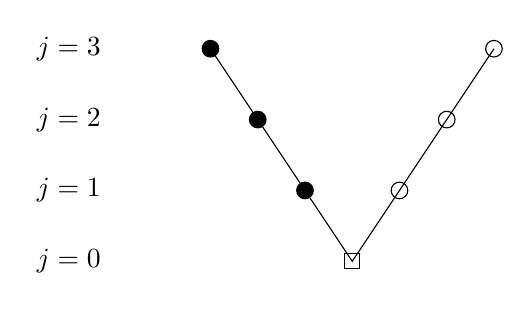
\begin{tikzpicture}[scale=1.2]
  \pgfmathsetmacro\hstep{0.5}
  \pgfmathsetmacro\vstep{0.75}
  \pgfmathsetmacro\ceps{0.08}   % size of square for coarse grid

% grid labels at left
  \node at (-2,3*\vstep) {$j=3$};
  \node at (-2,2*\vstep) {$j=2$};
  \node at (-2,\vstep) {$j=1$};
  \node at (-2,0.0) {$j=0$};

% V-cycle
  \draw[black,thin] (-\hstep,3*\vstep) -- (0.0,2*\vstep) -- (\hstep,\vstep) --  (2*\hstep,0.0)
                    -- (3*\hstep,\vstep) -- (4*\hstep,2*\vstep) -- (5*\hstep,3*\vstep);
  \filldraw (-\hstep,3*\vstep) circle (2.5pt);
  \filldraw (0.0,2*\vstep) circle (2.5pt);
  \filldraw (\hstep,\vstep) circle (2.5pt);
  \draw     (2*\hstep-\ceps,-\ceps) rectangle (2*\hstep+\ceps,+\ceps);
  \draw     (3*\hstep,\vstep) circle (2.5pt);
  \draw     (4*\hstep,2*\vstep) circle (2.5pt);
  \draw     (5*\hstep,3*\vstep) circle (2.5pt);
\end{tikzpicture}

\caption{A V-cycle on a three-level hierarchy ($K=2$) with a down-smoother (solid dots), up-smoother (circles) and coarse-level solver (square).}
\label{fig:vcycle}
\end{figure}

The above \textsc{vcycle} algorithm also calls a coarse solver on the $k=0$ level.  For a linear problem like our current Poisson problem it is traditional to apply a direct solver for this linear system (i.e.~equation \eqref{eq:linearsystem}).  However, this will not be an option for the nonlinear glacier geometry problem.  Instead we suppose \textsc{coarsesolve} is implemented as a fixed number of GS sweeps.  If the coarsest mesh has a single node then a single sweep gives an exact solution.

We have now presented a basic geometric multigrid algorithm via a particular FE viewpoint, namely the subspace decomposition approach as pioneered by Xu \cite{Xu1992} and others, an idea which applies both to multilevel and domain-decomposition algorithms.  We could now show computational results prominently featuring the efficiency of the V-cycle algorithm, namely evidence of optimal $O(m_K)$ time to solve the problem, and indeed such results appear in multigrid references \cite{Briggsetal2000,Bueler2021,Elmanetal2014,Trottenbergetal2001}.  However, we first introduce a less-trivial ``obstacle'' problem which has the essential free-boundary character of the glacier geometry problem.  Computational results will be given in the next three sections.


\section{Multilevel subset decomposition for the classical obstacle problem} \label{sec:obstacle}

\subsection*{An ice-like model problem}  We now have a basic view of the ``classical'' geometric multigrid (GMG) method from the multilevel subspace decomposition point of view.  However, as noted in section \ref{sec:intro}, the main problem in glacier modeling, of how the ice geometry and velocity co-evolve in response to climatic inputs, needs an inequality constraint for well-posedness.  The fact that the ice surface elevation must be above the bed generates the land-terminating boundary condition for the mass conservation problem.  Regardless of the manner in which momentum conservation (stress balance) is modeled, this inequality constraint by itself makes the problem nonlinear.  It also reduces solution regularity in a manner which is challenging to numerical methods.  (They are further-challenged by the non-Newtonian viscosity of the fluid.)

To address such inequality constraints, and before actually modeling glaciers in section \ref{sec:sia}, we introduce a more-convincing model problem, namely the classical 1D \emph{obstacle problem}.  This simply adds an inequality constraint to the same linear differential equation, the Poisson equation.  After stating the weak form, which is solved over a \emph{subset} of the function space in section \ref{sec:subspace}, we will modify the multilevel subspace decomposition approach to be a \emph{subset decomposition} method.  Each mesh level will host an inequality-constrained problem, and together all the levels will capture the original constraint set.  Switching the differential equation to the nonlinear SIA model in section \ref{sec:sia} will be comparatively an easy change.

We use the same domain $[0,1]$ and solution space $\mathcal{H}$ as the Poisson problem \eqref{eq:poisson}.  Recall that functions in $\mathcal{H}=H_0^1[0,1]$ are smooth and satisfy zero boundary conditions.  Let $\phi(x)$ be a fixed function, also in $\mathcal{H}$, which is the obstacle.  The strong form of our classical obstacle problem is a \emph{complementarity problem} (CP) \cite{Bueler2021,KinderlehrerStampacchia1980} which says that the Poisson equation applies whereever the solution $u(x)$ is strictly above the obstacle:
\begin{align}
  u - \phi &\ge 0 \label{eq:obstaclecp} \\
  -u''-f &\ge 0 \notag \\
  (u-\phi)(-u''-f) &= 0 \notag
\end{align}
The last condition, complementarity, implies that for each $x$ in $[0,1]$ the solution is on (coincides with) the obstacle, $u(x)=\phi(x)$, or the Poisson equation holds in an open set around $x$ (i.e.~$-u''(x)=f(x)$).  (Or both, but in the generic \emph{nondegenerate} \cite{KinderlehrerStampacchia1980} case the obstacle does not itself solve the Poisson equation.)  Conditions \eqref{eq:obstaclecp} also say that in an open set where the solution coincides with the obstacle, the source term is bounded above: $u=\phi \implies f \le -\phi''$.  Note that the solution $u$ and the obstacle $\phi$ are defined on the entire domain, but the (Poisson) differential equation only holds in the \emph{inactive} portion where $u>\phi$.  In the complementary region where $u=\phi$, the constraint is said to be \emph{active}.

As we will see in section \ref{sec:sia}, for the glacier problem there will also be a CP formulation.  The obstacle will be the bed elevation, the solution will be the glacier surface elevation, and the source term will be the climatic (surface) mass balance.  The CP formulation will say that the mass conservation equation holds on the glacier, and that off the glacier the surface mass balance is not positive \cite{Bueler2016}.

Returning to our classical obstacle problem, simply by choosing a source term $f(x)$ which is positive in the middle of the domain and negative near the boundaries, we get the ``ice-like'' solution shown in Figure \ref{fig:icelike}.  In detail, the Figure shows the exact, piecewise-quadratic solution $u(x)$ for the following data:
\begin{equation}
\phi(x) = x(1-x) \quad \text{ and } \quad f(x) = \begin{cases} 8, & 0.2 < x < 0.8, \\
                                                               -16, & x<0.2 \text{ or } x>0.8. \end{cases}  \label{eq:icelikedetails}
\end{equation}
(Note that $f$ is in $L^2[0,1]$ and it is defined almost everywhere.)  Finding the formula for $u(x)$, which smoothly-connects five rational-coefficient quadratic pieces, is an exercise for the reader.\footnote{Find the solution in: \, \href{https://github.com/bueler/mg-glaciers/blob/master/py/obstacle.py}{\texttt{github.com/bueler/mg-glaciers/blob/master/py/obstacle.py}}.}

% regenerate:
%   $ cd py/
%   $ ./obstacle.py -plain -kfine 5 -o icelike.pdf
%   $ pdfcrop icelike.pdf icelike.pdf
\begin{figure}
\includegraphics[width=0.7\textwidth]{fixfigs/icelike.pdf}
\caption{An ice-like configuration of the classical obstacle problem.}
\label{fig:icelike}
\end{figure}

Observe that the solution $u$ does not depend linearly on the source function $f$.  In fact, if $f(x)\le 0$ for all $x$ in $[0,1]$ then the solution to the problem with $\phi(x)=x(1-x)$, i.e.~the obstacle shown in Figure \ref{fig:icelike}, is $u=\phi$ on $[0,1]$.  For example, if $\tilde u$ solves the problem for $\tilde f= -1$, then $2\tilde u$ \emph{does not} solve the problem for source term $2\tilde f = -2$.  In this sense the classical obstacle problem is nonlinear even though the corresponding PDE, the Poisson equation, is linear.

\subsection*{Weak formulation with constraints}  For an FE method we will need the weak form of the problem.  Again it arises from multiplying by a test function $v$ and integrating by parts, but now the solution (and test-function) space incorporates the constraint:
\begin{equation}
\mathcal{K} = \left\{v \text{ in } \mathcal{H} \text{ such that } v \ge \phi\right\}.  \label{eq:Kdefine}
\end{equation}
This subset of $\mathcal{H}$ is not a vector space, but it is closed and \emph{convex}.  (This means that if $v,w$ are in $\mathcal{K}$ then any point on the line segment connecting them, namely $\alpha v + (1-\alpha) w$ for $0 \le \alpha \le 1$, is also in $\mathcal{K}$.)  Note that if $u$ solves problem \eqref{eq:obstaclecp} then $u$ is in $\mathcal{K}$.

The inequalities in \eqref{eq:obstaclecp} enter nontrivially into the weak-form derivation, not given here but found in \cite{Bueler2021,KinderlehrerStampacchia1980}, and the result is a single \emph{variational inequality} (VI):
\begin{equation}
  a(u,v-u) \ge \ip{f}{v-u} \quad \text{ for all } v \text{ in } \mathcal{K}. \label{eq:obstaclevi}
\end{equation}
Compare equation \eqref{eq:weakpoisson}; the bilinear form is the same: $a(u,v) = \int_0^1 u'(x) v'(x)\,dx$.  Inequality problems \eqref{eq:obstaclecp} and \eqref{eq:obstaclevi} are equivalent up to the same regularity concerns which relate the strong and weak forms of a PDE, respectively.  See reference \cite{Evans2010} regarding the solution regularity of PDEs, and \cite{KinderlehrerStampacchia1980} for the corresponding VI concepts.

The intuition behind a VI is often obscure and a barrier to understanding.  To help, we mention yet another weak form for the classical obstacle problem.  Inequality \eqref{eq:obstaclevi} is equivalent to \emph{constrained minimization}:
\newcommand{\argmin}{\mathop{\mathrm{arg\text{-}min}}}
\begin{equation}
  u = \argmin_{v \text{ in } \mathcal{K}} J(v) \quad \text{where} \quad J(v) = \frac{1}{2} a(v,v) - \ip{f}{v}. \label{eq:obstaclemin}
\end{equation}
That is, $u$ is the minimizer, over the constraint set $\mathcal{K}$, of the quadratic \emph{objective} functional $J$.  (The proof of equivalence is standard in continuous optimization; see \cite{KinderlehrerStampacchia1980} or \cite[Chapter 12]{Bueler2021}.)

The gradient of the objective $J$, at input $u$, defines the linear functional which appears in \eqref{eq:obstaclevi}.  In fact, the VI can be re-stated as follows:
\begin{equation}
  \nabla J(u)[v-u] \ge 0 \quad \text{ for all } v \text{ in } \mathcal{K}. \label{eq:obstaclevigradient}
\end{equation}
Thus the solution $u$ sits at a location in $\mathcal{K}$ where a vector pointing further into the constraint set, namely $v-u$ for $v$ in $\mathcal{K}$, points ``uphill'' on the graph of $J$.  If we think of $\nabla J(u)$ as a vector, instead of a linear functional, we could write \eqref{eq:obstaclevigradient} as $\ip{\nabla J(u)}{v-u} \ge 0$; this says that the angle between $\nabla J(u)$ and $v-u$ is at most 90 degrees.  While the VI always holds, one possibility is that the constraint $u\ge \phi$ is nowhere active on the domain, in which case \eqref{eq:obstaclevigradient} implies the unconstrained minimum condition $\nabla J(u)[v] = 0$ for all $v$ in $\mathcal{H}$; in that case the gradient of $J$ is zero at $u$.

To propose a more global mental image, imagine the constraint set $\mathcal{K}$ as analogous to the closed first quadrant in the plane, $\mathcal{Q} = \left\{(x_1,x_2)\,:\,x_i\ge 0\right\}$, and $J$ as analogous to a smooth, concave-up (i.e.~\emph{coercive} \cite{Evans2010}), objective function $\gamma(x_1,x_2)$ defined on $\mathcal{Q}$.  The solution $(\hat x_1,\hat x_2)$ in $\mathcal{Q}$, of the corresponding variational inequality or constrained minimization problem, may not be at a location where $\nabla \gamma$ is zero.  However, it will be as low as possible, even if that means it is hard against a boundary of $\mathcal{Q}$.  At this solution point all directions into $\mathcal{Q}$ will increase the value of $\gamma$, as sketched by contours in Figure \ref{fig:cartoonplane}.

The VI solution shown in Figure \ref{fig:icelike} is an infinite-dimensional version of the solution point shown in the cartoon view in Figure \ref{fig:cartoonplane}.  The glacier problem in the next section will analogously be formulated as a CP like \eqref{eq:obstaclecp} and as a VI like \eqref{eq:obstaclevi}.  However, for general bed elevation functions (obstacles) the glacier problem has no constrained minimization formulation like \eqref{eq:obstaclemin}; the essential reason is the lack of symmetry of the weak form in the general case \cite{JouvetBueler2012}.  We will return to this point in section \ref{sec:sia}.

\begin{figure}
\includegraphics[width=0.35\textwidth]{genfigs/cartoonplane.pdf}
\caption{For analogy purposes only:  A 2-dimensional constrained-minimization solution in a planar quadrant, with objective function contours.}
\label{fig:cartoonplane}
\end{figure}

Regardless of the way the classical obstacle problem is formulated, whether as \eqref{eq:obstaclecp}, \eqref{eq:obstaclevi}, or \eqref{eq:obstaclemin}, a \emph{free boundary} generally arises in the interior of the domain.  For example, in Figure \ref{fig:icelike} there are locations near the ends of $[0,1]$ where the solution becomes fully in contact with the obstacle.  At these locations both $u=\phi$ and $u'=\phi'$ hold, that is, the solution is tangent to the obstacle.  This free boundary involves simultaneous Dirichlet and Neumann ``conditions'' at a location which must be found as part of the solution.  Note that, in addition, there are the fixed boundary conditions from requiring the solution $u$ to be in the vector space $\mathcal{H}$.

Because of the free boundary, the solution of the classical obstacle problem can be non-smooth even when the data is arbitrarily smooth.  For example, smoothing the source term $f$ in \eqref{eq:icelikedetails} would give a solution nearly the same as shown in Figure \ref{fig:icelike}.  That is, one would make the source term $f$ into a smooth function by ``mollification'' \cite{Evans2010}; the transition between the positive interior value to the negative value would be $C^\infty$.  However, the free boundary would remain, and at that free boundary the second derivative $u''$ would jump from value $+16=-f$ to value $-2=\phi''$.  This is a case of the theorem that the solution for smooth data is limited to the Sobolev space $W^{2,\infty}$ \cite{KinderlehrerStampacchia1980}, and generically not smoother.

\subsection*{Constraint decomposition}  PGS first FIXME

We solve the classical obstacle problem by a \emph{constraint decomposition} \cite{Tai2003} method, which modifies the subspace decomposition to allow an inequality constraint.  FIXME

FIXME cite for multigrid obstacle \cite{BrandtCryer1983,Bueler2021,GraeserKornhuber2009,Jouvetetal2013}; cite for subset decomp \cite{Tai2003}

FIXME Figure \ref{fig:icelikedecomposition} shows the constraint decomposition;  Compared to Figure \ref{fig:icelike}, the obstacle $\phi$ is changed to have smooth ``topography''.

%REGENERATE Figures \ref{fig:icelikedecomposition} and \ref{fig:gooddecomposition}:
%$ ./obstacle.py -kfine 5 -irtol 1.0e-7 -random -randommodes 8 -diagnostics -up 0 -o defect.pdf
%fine level 5 (m=63) using 52 V(1,0) cycles (102.375 WU)
%saving final iterate and obstacle to defect.pdf ...
%saving residual and inactive residual to resid_defect.pdf ...
%saving hierarchical decomposition to decomp_defect.pdf ...
%saving "ice-like" decomposition to icedec_defect.pdf ...
\begin{figure}
\includegraphics[width=0.7\textwidth]{fixfigs/icedec_defect.pdf}
\caption{The multilevel constraint decomposition, visualized as a decomposition of the gap between the current iterate $w$ and the obstacle $\phi$.}
\label{fig:icelikedecomposition}
\end{figure}

FIXME Figure \ref{fig:gooddecomposition} shows the same decomposition as in Figure \ref{fig:icelikedecomposition}, but correctly; each level is piecewise-linear on its mesh level

\begin{figure}
\includegraphics[width=0.75\textwidth]{fixfigs/decomp_defect.pdf}
\caption{The constraint decomposition writes the fine-mesh defect obstacle $\phi - w$ as a sum of the gaps $\phi^k = \chi^k - \chi^{k-1}$ between the defect obstacles $\chi^k$ on each level.}
\label{fig:gooddecomposition}
\end{figure}

\subsection*{Results} FIXME


\section{Multigrid for a shallow-ice mass conservation problem} \label{sec:sia}

FIXME model problem in previous section has the wrong ``physics'' but correctly addresses the free boundary and obstacle nature of the glacier problem

FIXME cite for glaciers as obstacle problems \cite{Bueler2016,Bueler2020,Calvoetal2002,JouvetBueler2012}

FIXME for 2D domains the coarse mesh construction needs reconsideration


\section{Multigrid for a Glen-Stokes glacier flow} \label{sec:stokes}

FIXME multigrid already used for Blatter-Pattyn model \cite{BrownSmithAhmadia2013} and for hybrid \cite{Jouvetetal2013}; one goal of this section is to make these approaches more understandable

FIXME we use Schur complement \cite{Bueler2021,Elmanetal2014} and compare it to Vanka monolithic smoother \cite{Farrelletal2019}

\small

\bigskip
\bibliography{review}
\bibliographystyle{siam}

\normalsize
%\clearpage

\appendix
\section{Notation}

\renewcommand{\arraystretch}{1.2}
\begin{longtable}{l|l}
\textbf{Symbol} {\Large$\strut$} & \textbf{Meaning} \\ \hline
$a(\cdot,\cdot)$ & bilinear form associated to the Poisson problem; left side of equation \eqref{eq:weakpoissonearly} \\
$\mathcal{H}$ & Hilbert space for the continuum problem \\
$J$ & scalar-valued objective function, e.g.~$J(v) = \frac{1}{2} a(v,v) - \ip{f}{v}$ for the Poisson equation \\
$k$ & index of level in multilevel scheme; $k=0,1,\dots,K$ from coarse to fine \\
$\mathcal{K}$ & constraint (admissible) subset; $\mathcal{K} \subset \mathcal{H}$; e.g.~$\mathcal{K} = \{v \ge \phi\}$ \\
$\mathcal{K}^k$ & $k$th-level admissible functions; $\mathcal{K}^k \subset \mathcal{V}^k$ \\
$\ell[\cdot]$ & linear functional, e.g.~$\ell[v] = \ip{f}{v}$ \\
$m_k$ & number of nodes in $k$th-level; $\dim \mathcal{V}^k=m_k$ \\
$P$ & canonical prolongation of functions; equation \eqref{eq:canonicalprolongation} \\
$R$ & canonical restriction of linear functionals; equation \eqref{eq:canonicalrestriction} \\
$r(w)[\cdot]$ & residual of iterate $w$, e.g.~$r(w)[v] = \ip{f}{v} - a(w,v)$ for the Poisson equation \\
$\mathcal{V}^h$ & finite element function space; $\mathcal{V}^h = \mathcal{V}^K$ \\
$\mathcal{V}^k$ & $k$th-level vector space \\
$(\mathcal{V}^k)'$ & dual of $k$th-level vector space ($=$ linear functionals) \\
$x_p^k$ & $p$th node on $k$th-level mesh \\
$\phi$ & obstacle in continuum problem; $\phi \in \mathcal{H}$ \\
$\psi_p^k(x)$ & $k$th-level hat function at $x_p$ \\
$\ip{\cdot}{\cdot}$ & $L^2$ inner product \\
$\|\cdot\|$ & $L^2$ norm; $\|f\|=\ip{f}{f}^{1/2}$
\end{longtable}

\end{document}
